\documentclass{article}
\renewcommand\refname{Referencias}
\renewcommand\contentsname{\'Indice de Conten\'ido}
\usepackage{graphicx}
\graphicspath{{IMG/}}
\usepackage{caption}
\usepackage{subcaption}
\usepackage{float}
\usepackage{listings}
\lstset{
 showstringspaces=false,
 tabsize=2,
 frame=single,
 numbers=left,
 language=Pascal
}

\title{\textsc{Paradigmas y Lenguajes de Programaci\'on\\Trabajo Pr\'actico N\'umero 2\\-- Pr\'actica --}}
\author{Ulises C. Ramirez [uli.r19@gmail.com]\\H\'ector Chripczuk\\Ver\'onica Gonzalez}
\date{23 de Septiembre, 2018}

\begin{document}
\maketitle
\pagenumbering{gobble}
\newpage
\section*{Versionado}
Para el corriente documento se est\'a llevando un versionado a fin de mantener un respaldo del trabajo y adem\'as proveer a la c\'atedra o a cualquier interesado la posibilidad de leer el material en la \'ultima versi\'on disponible.\\

\begin{center}
  \textsc{Repositorio}: \textit{https://github.com/ulisescolina/UC-PYLP}
\end{center}


\hfill--\textsc{Ulises}\tableofcontents
\pagenumbering{gobble}
\newpage

% === Inicio del Cuerpo del Documento === %
\pagenumbering{arabic}
\section{Grafo de Precedencias}
\label{sec:}
\textsc{Consigna}: \textbf{Dado el fragmento de programa concurrente en el \texttt{Listing \ref{graprec}} obtener el grafo de precedencia asociado}.

\begin{lstlisting}[caption={Fragmento de programa concurrente}, label=graprec]
P0;
COBEGIN
	P1;
	P2;
	COBEGIN
		P3; P4; P5; P6;
	COEND
	P7;
COEND
P8;
\end{lstlisting}

A continuaci\'on se presenta el grafo de precedencia, la justificaci\'on del \textit{por qu\'e} se realiz\'o de esa manera tiene  sus bases en dos cuestiones mencionadas en el cursado de la materia.
\begin{itemize}
\item La primera de ellas tiene que ver con lo mencionado en \cite{gortazarbellas}, y expuesto adem\'as en una de las diapositivas de la c\'atedra y tiene que ver con el orden en el cual ocurre la ejecuci\'on de los diferentes procesos que se quiere paralelizar, en resumen, \'este acontecimiento es aleatorio, se elige un proceso al azar para que este se ejecute.
\item la otra parte, se expuso en clases durante la explicaci\'on de \textbf{qu\'e es un grafo de dependencias}, en donde se dejo constancia de que para que se pueda iniciar una tarea, debe ejecutarse, en primera instancia, la tarea fuente.
\end{itemize}


\begin{figure}[H]
  \centering
  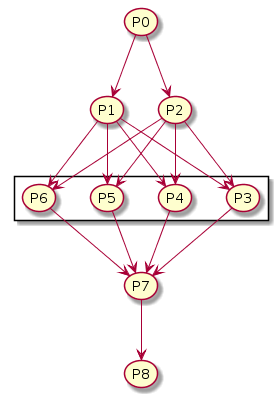
\includegraphics[width=.4\linewidth]{grafo_precedencia.png}
  \caption{Grafo de precedencia para \texttt{Listing \ref{graprec}}}
  \label{fig:graprec}
\end{figure}

En este caso tenemos a P1 y P2 como tareas fuente, las cuales deben finalizar, y de ah\'i se determina cual es la tarea es la siguiente, por lo expuesto en el primero de los dos puntos que se expusieron anteriormente, la selecci\'on sera al azar, por tanto se consideran todas los posibles escenarios de finalizacion de los padres.

% === Bilbiografia === %
\newpage
\begin{thebibliography}{99}
	% Item 1
	\bibitem[Gort\'azar Bellas, et al, 2012]{gortazarbellas}\textsc{Gort\'azar Bellas, Francisco; Mart\'inez Unanue, Raquel; Fresno Fern\'andez, Victor}. \textit{Lenguajes de Programaci\'on y Procesadores - Cap\'itulo 3.5}. Editorial Universitaria Ramon Areces, Madrid, 2012. \textsc{ISBN: 9788499610702}.
	% Item 2
	%\bibitem[Mattson, 2013]{mattson2013}\textsc{Tim, Mattson}. \textit{Introduction to OpenMP}. Intel. https://goo.gl/BZWNe3
\end{thebibliography}
\end{document}
